%% This is a skeleton file to create IEEE style Bibliography list. There is a guide added "create-manual-bib-entry.txt" to manually create popular types of references such as PhD thesis, website, unpublished work etc.
%%
%% Modified by K. Reaz( kahn.reaz@ieee.org)
%% Support sites:
%% http://www.ieee.org/

%%***********************************************************
%% Legal Notice:
%% This code is offered as-is without any warranty either expressed or implied; without even the implied warranty of MERCHANTABILITY or FITNESS FOR A PARTICULAR PURPOSE! 
%% User assumes all risk and can modify as s/he wants.

%%***********************************************************

%package list
\documentclass[journal]{IEEEtran}
\usepackage{cite}


\begin{document}

\author{Sean Jennings}
%Here goes the title
\title{Frequency Control for Inverter-based Resources}
\maketitle

\begin{abstract}
The abstract goes here.

This is a mf abstract!
\end{abstract}

%Main body starts
\section{Introduction}
%% Insert your citation key below as it is in main.bib file to generate References in IEEE format.
\IEEEPARstart{T}{he} penetration of renewable energy sources (RES)
projected to increase over the coming decades, with gains highly powered by
solar and wind resources. The NREL 
has solar and wind energy increasing to $>$50\% share by 2050
\cite{lin_research_2020}. 
Solar photovoltaics (PV) and Type III and Type IV wind turbine generators
(WTG) are both inverter-based resources (IBRs), in contrast to
synchronous generators (SGs) of which the conventional power grid is
mostly composed.

Throughout the history of the power grid, reliability has been a prime concern.
A core aspect of power system reliability is frequency control, the ability
to maintain the AC voltage and current signals close to a given setpoint
(e.g. 60 Hz in the USA) \cite{anderson_power_2003}. If frequency deviates too far from its setpoint,
protection mechanisms of the grid, such as under-frequency load shedding
(UFLS) are triggered to prevent damage to equipment and to arrest further
instability \cite{denholm_inertia_2020}
Load shedding means that some customer(s) have lost power, a serious grid
reliability issue.


When the grid is near equilibrium, its frequency is closely related
to the real power transfer between its nodes. When a system fault, such as a
generator going offline, causes a power imbalance in the system, 
the rest of the generators increase power output to balance
generation and load. To transfer power between nodes requires the phase angle
between nodes in the system to shift, which results in transient frequency
deviations.

The rate at which frequency changes (RoCoF) is related to underlying physical
system from which the energy is derived. Conventionally,
thermal power plants use SGs to convert the underlying mechanical energy
contained in steam into electrical energy. The RoCoF is limited by
the mechanical {\bf inertia} of the SG as governed by the swing equation.

On the other hand, IBRs connect an energy resource such as a PV cell,
WTG, or a battery energy storage system (bESS) to the grid via a 
power electronic (PE) inverter which converts a DC source to an AC output.
The dynamics governing the energy resource as well as the control algorithm.
Because the IBR is not directly connected to any form of mechanical inertia,
IBR do not have inertia and that systems with high penetrations of IBRs
are {\it low-inertia} systems.

The control algorithms used by IBRs can be broadly divided into two strategies:
\begin{enumerate}
  \item Grid-following Inverters (GFL), and
  \item Grid-forming Inverters (GFM).
\end{enumerate}

While the IEEE has established standards for GFL converters \cite{photovoltaics_ieee_2018},
the definition of GFM remains debated within research communities.
To date, there is no IEEE standard on the definition of GFM.
NREL defines a GFM to be any inverter that does not operate with a phase-lock loop (PLL)
\cite{lin_research_2020}

There has been some debate on the security of IBRs. The authors
of \cite{milano_foundations_2018}
posit that "low inertia likely implies low security" since
lack of mechanical inertia means that the stability of the system
relies on the software implementation of control algorithms. Thus,
there is a growing body of research aimed at demonstrating the 
robustness of the control strategies deployed on IBRs.

Despite the informal definition, GFM control technology is
not new: since the 1990s, it has been researched extensively by
the microgrid research community \cite{lin_research_2020},
and implemented within smaller power systems. However, the 
integration of GFM systems into the power grid on a larger scale
has 

While the deployment of increasing penetrations of IBR to the large-scale
grid may not be gauranteed, it remains one of the currently most 
economically feasible paths to net-zero carbon emissions. Furthermore,
any potential deployment will necessarily be gradual process: the entirety of
SG-based generation cannot be replaced with generation based on IBRs
overnight. Therefore, it is of vital importance to study the 
dynamics of IBR-based frequency control in the variety of contexts
anticipated in the forthcoming energy transition. Since this
entails nothing less than a complete rearchitecting of the energy
grid, there are numerous open research questions in this field
which will be enumerated.

This literature review focuses on the challenges and oppurtunities along
the path to incorporating high levels of IBR penetration into the grid 
at a large scale. It is organized as follows: section \ref{sec:math-models}
summarizes the mathematical formulation for frequency control; section
\ref{sec:control-strategies} enumerates and classifies the many
of control schemes that have been proposed in literature; section
\ref{sec:commericial-demonstrations} summarizes the major commericial
projects which have been deployed using GFM technology to-date.



\section{A Mathematical Formulation for Frequency Control}


\label{sec:math-models}

\subsection{Synchronous Generators}
 We begin our summary of the literature by reviewing the dynamics of SGs, 
 which is a topic that has been well-established
 for decades. Despite it's lack of novelty, the topic remains highly
 relevant to the problem of IBR frequency control since
 \begin{enumerate}
  \item a substantial portion of the prevailing industry terminology
    is based around these terms, and
  \item SG dynamics interact with IBR dynamics via their network
    interconnections within the grid.
 \end{enumerate}

%  A SG is composed of three major components from a control standpoint,
% the excitation system, the 

 The relationship between power and frequency in a SG is governed by
 \begin{equation}
  J\dot{\omega} = p_m - p_e
  \label{eq:swing-equation}
 \end{equation}
 where $J$ is the system intertia, $p_m$ is the mechanical power input to
 the generator, and $p_e$ is the electrical power which is absorbed
 by connected loads.

Since a change in frequency signals there is a power imbalance within the
system, the rotor speed of an SG is typically regulated by a
feedback-mechanism called the governor. This feedback couples a change in 
frequency, $\omega$, to a (typically proportional) change in the power
delivered by the prime mover $p_m$:
\begin{equation}
  \dot{p_m} = - \frac{\omega_{set}}{R} * (\omega - \omega_{set}) + p_{m,set}
  \label{eq:governor-control}
\end{equation}

Combining equation \ref{eq:swing-equation} and \ref{eq:governor-control}
gives a second order relationship between frequency, $\omega$ and 
mechanical power delivered, $p_m$.
 
\subsection{IBR Grid Integration}
In contrast, the frequency-real power relation for IBR resources are not
coupled by mechanical inertia of the swing equation,
but rather are determined by the underlying energy source for the IBR system.
%\ref{interactivity}
defines makes the assumption that power and energy is available from a bESS,
but the same conclusions hold if the energy source is curtailed PV or wind power.
This assumption is a common and vital one: it informs the design of
the DC side of an IBR. %\ref{battery-sizing}
elaborates on the relationship between the control parameters and
the power requirements for the bESS.

%\ref{interactivity}
demonstrates that the timescale of IBR reactions are an order of magnitude
shorter than the mechanical timescale (~1 second) which SGs operate.
Thus, when considering the interaction between the two we find that 
% $p_{m,G} \approx p_{m,Go}$ is a
on this short timescale, the IBR response is first-order with respect to the
electrical power $p_{m,I}$ drawn from the circuit:
\begin{equation}
  \dot{p_{m,I}} = \frac{2 \pi (p_{e,I} - p_{m,I})}{\tau_I}
\end{equation}

It is well-documented that if the grid contains above a certain penetration
of GFLs, instability occurs. Therefore, for grids with high
IBR penetrations, a certain percentage of GFMs are necessary to maintain
stability. However, GFMs can also have their own drawbacks: they are
require more specialized hardware and control algorithms so are
therefore more expensive.

It has been shown that the placement of GFMs within a power system
topology has an important impact on overall system stability in a 
system with mixed GFL, SG, and GFM-based resources. However,
the exact interaction between GFLs and GFMs remains an open research
question. In particular, the ratio of GFLs to GFMs at which instability
arises and the optimal placement of GFMs within a given power system
remain under-studied questions.

A major difference between the physics of IBRs versus SGs is that
typically IBRs have a much lower current threshold that they
can produce based on the limits of the underlying PEs. As a result,
they have a smaller short-circuit ratio, which corresponds to 
a lower system strength. In general, a weaker system strength
implies a decrease in the voltage stiffness, which can impair
IBR performance. GFMs can provide "voltage strength" which is another
advantage over GFLs. Since this review is focused on frequency
control of IBRs, we will consider further discussion on the topic
as out of scope and will conclude with the note that voltage and
frequency control are inherently coupled and modeling these 
interactions is vital for demonstrating system stability.
\section{GFM Control Strategies}
\label{sec:control-strategies}

\begin{figure}
    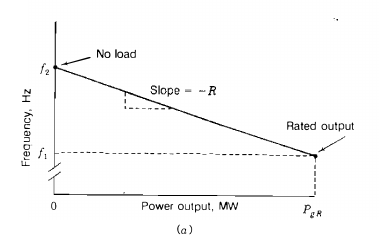
\includegraphics[width=0.8\linewidth]{Images/droop_control.png}
    \captionof{figure}{Linear droop control curve \cite{anderson_power_2003}}
    \label{fig:droop-control}
\end{figure}


The authors of \cite{lin_research_2020} propose the following categorization
of GFM control strategies:
\begin{enumerate}
  \item droop control
  \item virtual synchronous machine (VSM)
  \item virtual oscillating control (VOC)
\end{enumerate}
but they also note that these various strategies share properties in common.
In particular, for all these control strategies, the GFM inverter acts
as a voltage source.

\subsection{Droop Control}
"Droop control" is a term inherited from the classical literature on
SGs, where it presumably refers to the "droop" of the mechanical centrifugal governor
control mechanism. According to \cite{anderson_power_2003},
droop is defined as the relationship
between a generator's change in frequency as the power output varies from no load
to the rated output, per the following equation
\begin{equation}
    R_{pu} = \frac{\delta \omega_{pu}}{P_{rated,pu}}
\end{equation}
where $\delta \omega_{pu}$ is the per-unit change in frequency, $P_{rated,pu}$ is
the per-unit rated power, and $R_{pu}$ is the per-unit droop.

Within the GFM technology, this is the most well-established
control techniques, see \cite{chandorkar_control_1993}. Typically, a linear droop relationship is established
according to
\begin{equation}
  \omega^* = \omega_0 - R (P_* - P)
\end{equation}
where $\omega_*$ is the frequency setpoint of the system, $\omega_0$ is the nominal
frequency, $R$ is the droop characteristic, $P_*$ is the power setpoint, and $P$
is the actual current power (adapted from \cite{chandorkar_control_1993}). The
relative $R$ values throughout the system then determine how power is shared
between devices. Figure (\ref{fig:droop-control})

Recent studies have investigated "nonlinear droop control" which establish a nonlinear
relationship between frequency and real power output. \cite{kenyon_droop-e_2022}
proposes an algorithm called "Droop-e" in which frequency and power are related
by an exponential curve, which "allows greater utilization of available headroom."
In other words, since in any power system the generators must hold some power in reserve
in case of contingencies, a nonlinear relation can allow operation closer to
the system capacity. \cite{kenyon_interactive_2023} also compares various non-linear
droop controls in the mixed GFM/GFL systems. Figure (\ref{fig:droop-control-schematic})
displays a control schematic for a common droop controller.

\begin{figure}
    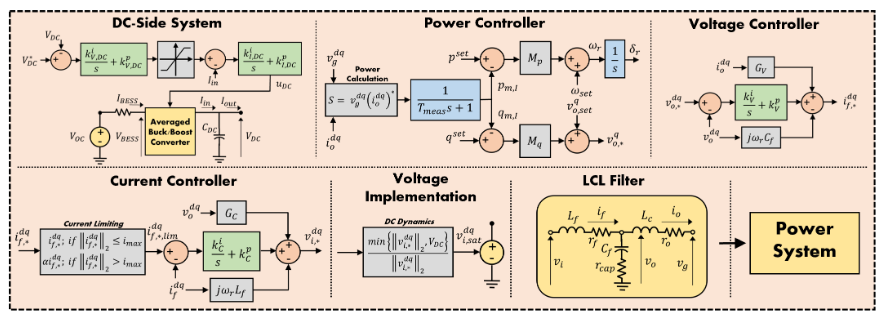
\includegraphics[width=0.8\linewidth]{Images/PE_control_layout.png}
    \captionof{figure}{Droop control schematic \cite{kenyon_interactive_2023}}
    \label{fig:droop-control-schematic}
\end{figure}


\subsection{Virtual Inertia-based Schemes}
Both VSM  strategies aim to emulate SGs by designing controllers
which exhibit similar dynamical properties to an SG. Namely, they 
attempted to emulate the mechanical inertia of SGs, commonly referred
to as virtual inertia (VI).
These methods ensure that the RoCoF after a distrubance remains constrained
within a certain limit. This is important because various components of
power system protection make assumptions on RoCoF, so that changes
in the dynamical properties of underlying generation may invalidate
protection-related assumptions \cite{denholm_inertia_2020}.

\begin{figure}
    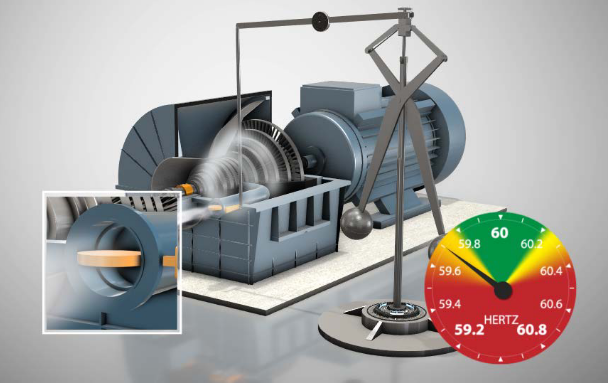
\includegraphics[width=0.8\linewidth]{Images/synchronous_generator.png}
    \captionof{figure}{Inertia and control of synchronous generator \cite{denholm_inertia_2020}}
    \label{fig:synchronous-generator}
\end{figure}

The degree to which it is possible to fully emulate an SG is again driven by 
the physics of the underlying system. For instance, due to the relatively
limited current that PEs, differences in behavior between SG and
VSM-controlled PEs can emerge during fault scenarios \cite{milano_foundations_2018}.
However, VSM control algorithms can provide a good baseline for control algorithm
performance.

It is generally agreed upon that virtual-inertia-based techniques, while serving
as a good starting point are inherently limited in performance since they do not
take capitalize on one of the main advantages of PEs, much faster response times
than SGs \cite{milano_foundations_2018}. \cite{kenyon_interactive_2023} shows
in simulation that although systems with GFMs exhibit faster RoCoF, they also
are able to reduce the maximum deviation from the nominal frequency. 

% \subsection{Optimization-based techniques}

% [TODO: foundations and challenges paper has interesting notes on optimal
% control parameter tuning, etc., read this more thoroughly!]

\section{Commercial Demonstrations of GFM technology}
\label{sec:commericial-demonstrations}

This section analyzes the scientific documentation of the
current state of the GFM industry's commercial development,
with the objective of illuminating the degree to which
the control strategies and system models of sections
\ref{sec:math-models} and \ref{sec:control-strategies}
have been tested and validated on physical systems rather
than simply simulation.

\subsection{Distributed IBRs}
The IBRs which have been deployed to-date within
distributed (rooftop) PV \cite{noauthor_grid_2021} and WTG \cite{nguyen_grid-forming_2022}
have been primarily GFL technology. As discussed in section \ref{sec:grid-integration}
converting a GFL IBR to a GFM IBR requires upgrading
the hardware itself, along with a high capital cost. The projected
increase in GFL penetration makes the understanding the relationship
between GFL and GFM dynamics an even more pressing topic.

\subsection{Microgrids}
The Maui power system is a commonly used example of a MG which has 
high instantaneous power of IBRs \cite{kenyon_criticality_2023}.
Other small-scale grids (e.g. grids on small islands) have demonstrated the technical
feasibility of GFM technology \cite{lin_research_2020} while simultaneously presenting 
discrepancies from existing simulation results \cite{kenyon_criticality_2023}.

\subsection{Utility/Grid-scale Implementations}
The authors of \cite{musca_grid-forming_2022}
provide a recent overview of grid-scale systems which have implemented GFM
technology. The reviewed GFM pilot projects typically control a "hybrid power plant,"
consisting of combined solar, wind and battery resources, and are integrated with the grid
on the transmission-level.

The 14 project highlighted by this paper were all completed after 2012, demonstrating
the novelty of large-scale GFM installations. The authors of \cite{musca_grid-forming_2022}
also note that pilot projects represent a valuable source of data for validating
the fidelity of GFM modeling studies.
\section{Conclusion}
Given the projected rapid growth in IBRs, the instability of a
zero-inertia system based entirely off of GFL technology, as well
as the current rapid deployment of GFL technology, there is a clear
necessity for standards and commericalization of GFM technoogy.

A prerequisite for such standards is thorough characterization
of the stability characteristics of hybrid power systems. The
large body of active research into GFM control algorithms
has provided many promising results for the technical feasibility.

Still, many questions remain. The author is particularly interested
in further investigating the relationship between PS topology, GFM/GFL
hybrid dynamics, as well as a more detailed understanding of the
convergence properties of various optimization-based control algorithms.


\bibliographystyle{IEEEtran}
\bibliography{main}

\end{document}